\lesson{1}{Oct 6 2021 Wen (07:20:33)}{Atomic Theory}{Unit 2}

In the 1800s, gathering evidence for an atomic model was challenging. At that time tools didn't exist for scientists to get a good hard look at atoms. But that didn't stop \bf{John Dalton} from observing atomic behavior.
He devised a way to indirectly observe atomic nature using things he could measure and observe, such as

\begin{itemize}
    \item Temperatures
    \item Atmospheric conditions
    \item Weather patterns
\end{itemize}

Here are some of the things that he found:

\begin{definition}[All matter is composed of extremely small particles called atoms.]
    The word \bf{"atom"} comes from a Greek word meaning \bf{"cannot be cut into smaller pieces"}. Atoms have their own internal structure that can vary in mass and composition. The types of atoms that make up matter determine its properties.
\end{definition}

\begin{definition}[Atoms of a given element are identical in size, mass, and other properties.]
    An element is a substance that cannot be broken down into simpler substances.
    Atoms of a given element are identical. For example, all silver atoms are exactly the same.
    A silver atom may have some similarities with a gold atom, but there will always be some differences, such as mass or other properties.
\end{definition}

\begin{definition}[Atoms cannot be subdivided, created, or destroyed in chemical reactions.]
    According to the law of conservation of mass, matter cannot be created or destroyed. However, scientists will discover that atoms can be subdivided under unique circumstances.
\end{definition}

\begin{definition}[Atoms of different elements can combine in simple, whole-number ratios to form chemical compounds.]
    John Dalton's observations eventually led to the law of multiple proportions, which explains that atoms combine to form compounds in simple, whole-number ratios. For example, water is made of two atoms of hydrogen and one atom of oxygen. There's no such thing as a half atom within a compound.
\end{definition}

\begin{definition}[In chemical reactions, atoms are combined, separated, or rearranged.]
    The bonds between atoms are broken, rearranged, and reformed into new compounds during chemical interactions.
\end{definition}

There's only so much you can study about atoms from a macroscopic level. To understand the atomic nature of matter, scientists had to get microscopic. Let's take a closer look at the important atomic discoveries made by J. J. Thomson, Ernest Rutherford, Niels Bohr, and James Chadwick—no microscopes necessary.

\subsubsection*{1897-1906 -- Discovery of Electrons}

\paragraph{Experiment} J. J. Thomson loved working with cathode rays—the glowing beams of light we once used in television and computer screens. In 1897, after many cathode ray tests, J. J. Thomson discovered smaller, negatively charged particles inside the atom. He called them corpuscles because they were so small, but we now call them electrons.

\paragraph{Conclusion} Thomson hypothesized that these corpuscles were scattered within a positively charged atom, just like plums are mixed throughout plum pudding—hence the name of his model. (You may think of it as chocolate chips scattered in cookie batter.)

\subsubsection*{1908-1913 -- Rutherford and the Nucleus}

Ernest Rutherford was a student of J. J. Thomson, so he supported the plum pudding model. But he soon discovered that the model didn't quite fit.

\paragraph{Experiment} In Rutherford's experiments, he made observations about the behavior of positively charged particles as they were radiated onto a piece of gold foil. He noticed some of the particles did not pass straight through the foil as he expected. Some particles scattered, and some bounced back.

\paragraph{Conclusion} Rutherford proposed that there must be something big and positively charged in the center of each gold atom to cause the radiation particles to do this. He named this center the nucleus of the atom. He also proposed that the nucleus was composed of two particles, one that was positively charged (proton) and one that was neutral.

\subsubsection*{1913 -- Bohr's Orbitals}

\paragraph{Experiment} Niels Bohr worked with Ernest Rutherford on atomic structure. After observing the spectrum of colors that were emitted when a gas was excited (electrons gained energy), he believed the different wavelengths of color represented the energy levels an electron could exist within.

\paragraph{Conclusion} Bohr proposed that electrons moved in specific orbits around a positive nucleus based on their energy level. He predicted there were many energy levels in which electrons could exist. They are not randomly scattered, as scientists first predicted.

\subsubsection*{1927-1932 -- Chadwick and the Neutrons}

When he was only 19 years old, James Chadwick worked under Ernest Rutherford during his gold foil experiments. More than 20 years later, Chadwick isolated the neutral particle Rutherford had proposed. He called it the neutron.

\paragraph{Experiment} Chadwick found the neutron during his experiments in 1932. He and his fellow scientists bombarded beryllium atoms with alpha particles, and an unknown radiation was produced. It was composed of particles with a neutral electrical charge.

\paragraph{Conclusion} Chadwick was able to determine that the neutron existed in an atom's nucleus and that its mass was very close to the mass of a proton.

\subsubsection*{Crookes's Cathode}

Thomson's discovery of the electron would not have been possible without the experiments of Sir William Crookes. Crookes created an innovation called a cathode tube, which allowed electrically charged gas particles to flow between electrodes positioned at both ends of a sealed tube.

In one of his experimental investigations, Crookes placed an object within the path of the cathode ray. Turn on the cathode ray below, and observe what happens. What conclusion can be drawn from these results?

\subsubsection*{Thomson's Electrons}

The English physicist Sir J .J. Thomson conducted more experiments using cathode ray tubes. Use the cathode ray below to repeat some of the investigations Thomson conducted.

What do you think will happen if you place a negatively or positively charged rod near the cathode ray tube? What do you think will happen if a different element is used as the negative electrode in the cathode ray tube? Select each rod to view the experiments.

\subsubsection*{Rutherford's Nucleus}

Rutherford expected heavy, fast-moving alpha particles to be able to pass straight through a piece of thin gold foil without being affected by the atoms of gold. He assumed that Thomson's plum pudding model was accurate, that matter and mass were evenly distributed throughout the atom. If this model was correct, there should have been nothing to alter the course of the heavy particles flying through the foil.

\subsubsection*{Bohr's Quantum Model}

Rutherford expected heavy, fast-moving alpha particles to be able to pass straight through a piece of thin gold foil without being affected by the atoms of gold. He assumed that Thomson's plum pudding model was accurate, that matter and mass were evenly distributed throughout the atom. If this model was correct, there should have been nothing to alter the course of the heavy particles flying through the foil.

\subsubsection*{A Challenge to the Bohr Model}

For the most part, Bohr's model has been consistent with current research. However, there is a new model that adds to our understanding of atomic structure and electron behavior. The scientists Schrodinger and Heisenberg developed an alternate theory about atomic nature. Using calculations to determine electron position, they explained that electrons probably do not move in exact orbits like planets in a solar system. Instead, they exist in an electron cloud around the nucleus. They proposed that we can only predict the probable orbital path or position of electrons in an atom. Where the electron cloud is most dense, the probability of finding the electron is greatest.

\begin{marginfigure}
    \centering
    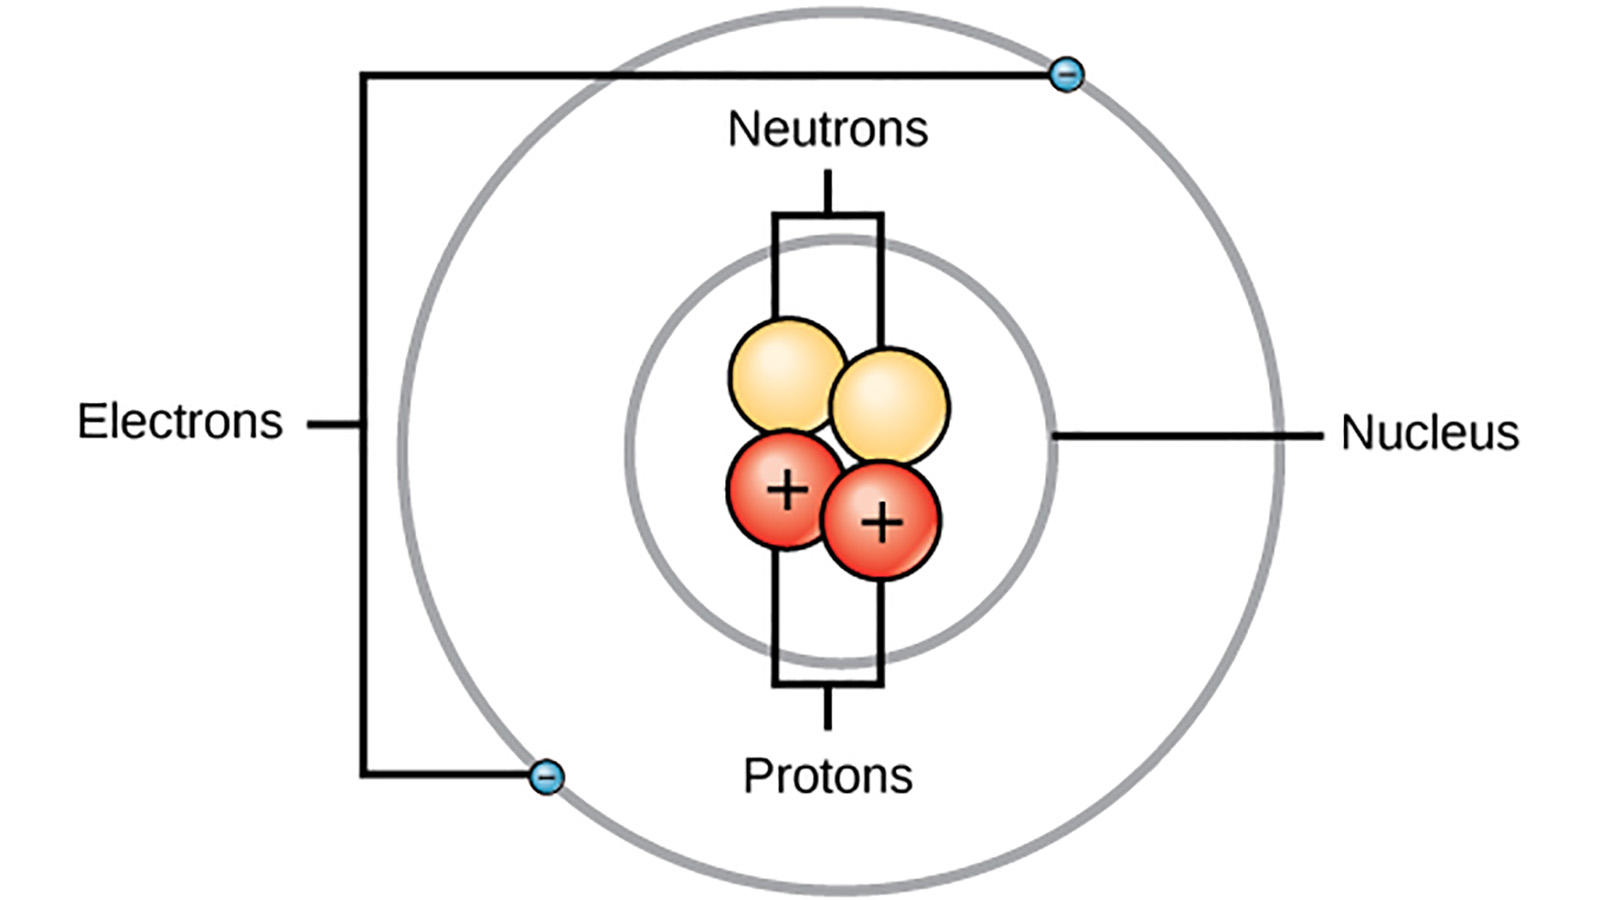
\includegraphics[width=\textwidth,height=\textheight,keepaspectratio]{images/bohr_model}
    \sidecaption{Image of the model.}
    \label{fig:bohr-model}
\end{marginfigure}

\subsubsection*{Parts of the Atom}

\paragraph{Proton} A neutral atom for the element lithium has three protons and three electrons. If one of its electrons happened to be removed from the electron cloud, then it would have three protons and two electrons. This greater number of protons would now make this entire atom a positively charged ion. It would attract negatively charged substances to it.

\paragraph{Electron} A neutral atom for the element oxygen has eight protons and eight electrons. If it happened to gain one electron from somewhere, then it would have eight protons and nine electrons. This greater number of electrons would now make this entire atom a negatively charged ion. It would be attracted to positively charged substances.

\paragraph{Neutron} Don't be tricked. Neutrons have no charge. If an atom has a greater number of neutrons than electrons and protons, and the numbers of electrons and protons are equal, then the atom is still neutral. It is possible for atoms of the same element to have different numbers of neutrons. These types of atoms are called isotopes. However, this does not affect the charge of the atom, only its mass.

\newpage
